\documentclass[11pt]{article}
\usepackage[T1]{fontenc}
\usepackage{lmodern}
\usepackage[margin=1in]{geometry}
\usepackage{amsmath,amssymb,amsthm,mathtools}
\usepackage{microtype}
\usepackage{enumitem}
\usepackage{booktabs}
\usepackage{xcolor}
\usepackage{tikz}
\usetikzlibrary{arrows.meta,positioning,calc,decorations.pathreplacing}
\usepackage[colorlinks=true,linkcolor=blue!45!black,citecolor=blue!45!black,urlcolor=blue!45!black]{hyperref}
\usepackage[nameinlink,noabbrev,capitalise]{cleveref}
\pdfinfoomitdate=1
\pdftrailerid{}
\pdfsuppressptexinfo=15
\numberwithin{equation}{section}
\newtheorem{theorem}{Theorem}[section]
\newtheorem{lemma}[theorem]{Lemma}
\newtheorem{proposition}[theorem]{Proposition}
\newtheorem{corollary}[theorem]{Corollary}
\theoremstyle{definition}
\newtheorem{definition}[theorem]{Definition}
\newtheorem{remark}[theorem]{Remark}
\newcommand{\OPT}{\operatorname{OPT}}
\newcommand{\pref}{\operatorname{pref}}
\newcommand{\suf}{\operatorname{suf}}
\newcommand{\len}[1]{\lvert #1\rvert}
\newcommand{\eps}{\varepsilon}
\newcommand{\ZZ}{\mathbb Z}
\newcommand{\NN}{\mathbb Z_{\ge0}}
\newcommand{\cost}{\operatorname{cost}}
\setlist{itemsep=3pt,topsep=5pt}
\emergencystretch=1em
\title{A Polynomial-Time 2-Approximation for\protect\\ Shortest Common Superstring}
\author{OpenAI}
\date{September 24, 2026}
\hypersetup{pdftitle={A Polynomial-Time 2-Approximation for Shortest Common Superstring},pdfauthor={OpenAI}}
\begin{document}
\maketitle
\begin{abstract}
We give a deterministic algorithm that, for every finite family of explicitly
represented ordinary strings, outputs a common superstring of length at most
twice the optimum in time polynomial in the total encoded input size, including
symbol labels. The guarantee applies to the algorithm constructed here, not the
classical maximum-overlap Greedy procedure.
\end{abstract}
\section{Introduction}\label{sec:intro}

In the \emph{shortest common superstring problem}, the input is a finite collection $\mathcal S$ of finite strings, and the task is to find a shortest string containing every member of $\mathcal S$ as a contiguous substring. Write $\OPT(\mathcal S)$ for its minimum possible length. The strings are represented explicitly, with encoded symbol labels and string boundaries. Let $N$ be the total bit length of this representation and $L$ the sum of the string lengths measured in symbols. Each symbol and boundary occupies at least one bit, so $L,|\mathcal S|\le N$; operations on symbol labels are charged for their encoded lengths.

\begin{theorem}\label{thm:main}
There is a deterministic algorithm, polynomial in the total encoded input size, that on every finite collection $\mathcal S$ of explicitly represented ordinary strings outputs a common superstring $T$ satisfying
\[
\len{T}\le 2\OPT(\mathcal S).
\]
\end{theorem}

\paragraph{History and significance.}
Tarhio and Ukkonen proposed the factor-$2$ conjecture for the maximum-overlap Greedy procedure~\cite{tarhio1988}. Blum, Jiang, Li, Tromp, and Yannakakis established a polynomial-time $3$-approximation~\cite{blum1994}; Sweedyk later obtained a $5/2$ guarantee~\cite{sweedyk1999}. Subsequent guarantees include $2+11/23$ due to Mucha~\cite{mucha2013} and $(14+\sqrt{67})/9<2.466$ due to Englert, Matsakis, and Vesel\'{y}~\cite{emv2023}. An August 2026 preprint of Chukhin, Kulikov, Mihajlin, and Smal reports a $7/3$-approximation~\cite{cycle2026}. \Cref{thm:main} answers affirmatively the question of whether a polynomial-time factor-$2$ approximation exists.

Many earlier approximation algorithms use the distance graph on the input strings, whose edge costs are the lengths of prefixes left after maximum suffix--prefix overlap. A minimum-weight cycle cover gives a computable lower bound, but its cycles must then be opened and joined while controlling the extra length~\cite{blum1994}. Breslauer, Jiang, and Jiang use rotations of periodic strings to control overlaps~\cite{breslauer1997}; Mucha sharpens this analysis through lexicographically extremal primitive rotations~\cite{mucha2013}. These provide conceptual precedents for the periodic comparisons below; our lower bound and the graph to which we apply them are different.

Our graph representation comes from another formulation. Golovnev, Kulikov, and Mihajlin introduced a hierarchical graph in the bounded-length setting~\cite{golovnev2014}, and the Collapsing framework developed its all-substrings form~\cite{collapsing2020}. In this graph, appending or deleting a letter gives an edge between substring vertices, and a superstring is represented by a closed walk visiting the required strings. The separation between a balanced graph and the operations that connect it also appears in the hierarchical cycle-cover discussion of that framework~\cite[revised version, Section~7.2]{collapsing2020}. We use this representation to turn forced occurrence counts into a balanced graph and then connect it within the same cost bound.

The factor-$2$ question has also motivated conjectures about specific procedures. The classical Greedy conjecture concerns repeatedly merging a pair of maximum overlap, while the Collapsing conjecture concerns a prescribed normalization of doubled hierarchical-graph walks~\cite{collapsing2020}. A September 2026 preprint of Shibata reports a counterexample to the Greedy conjecture, with worst-case ratio at least $9/4$~\cite{greedy2026}. Our theorem concerns the algorithm proved here; neither of those prescribed procedures is assumed to attain factor $2$.

\paragraph{Proof overview.}
The vertices of our hierarchical graph are all substrings of the inputs, including the empty word. An up edge appends a letter and costs one; a down edge deletes the first letter and costs zero. A balanced multiset of edges has equal incoming and outgoing degree at each vertex. If its support is connected and visits the empty word and every required string, an Euler tour spells a common superstring whose length is its up-edge cost.

We first construct integer counts $m(s)$ no larger than the number of occurrences of $s$ in any common superstring. Their one-letter sum $W$ is therefore a lower bound on the optimum. Counts for longer words constrain those of their prefixes and suffixes. A further rule handles periodic words. Relative to a fixed periodic text, a bracketing word consists of a matching interval with a mismatching letter at each end. When the assigned count of a long word exceeds the contribution of its bracketing words, a prefix shorter by $k$ periods must have count at least $k+1$ above its own bracketing contribution. The resulting counts determine a balanced, possibly disconnected graph of cost $W$.

Next decompose that graph into closed walks. The letters appended during a walk, repeated in both directions, form a periodic text; each visited vertex is a finite interval of that text. Walks with the same periodic text can be rearranged, preserving every edge, into ordered walks that each traverse one least period. We call these walks \emph{layers}. A layer of period $p$ has cost $p$ and receives a further budget $p$, so all additional budgets together equal $W$. In the remaining case of the connection procedure, the count rule forces a shorter word to occur on a layer with a different aligned text. A visited interval agreeing with both texts gives an actual graph vertex at which to attach a connection.

The final task is to arrange these connections without spending a budget twice. Some closed walks connect their source layers to a target using only the source budgets. Others require a contribution from the target, but these requests go only to a strictly larger period and are handled together when that period is processed. For each connection paid for only by its source layers, those layers can instead be joined internally while saving one period of budget. The remaining source-funded connections may form directed cycles. On each cycle, a maximal lexicographic rotation yields a contact word no longer than the target's period. Omitting that target's outgoing connection and joining its layers internally therefore pays for a round trip from the contact to the empty word. This connects the base graph at additional cost at most $W$ and completes the factor-$2$ bound.

\paragraph{Organization.}
\Cref{sec:counts} constructs the counts and their balanced graph. \Cref{sec:layers} develops the layer representation and the periodicity facts. \Cref{sec:connections} gives the connection operations, \Cref{sec:processing} processes groups of equal primitive text, and \Cref{sec:cycles} resolves the remaining cycles. \Cref{sec:algorithm} proves polynomial time and extracts the output string.

\section{Forced occurrence counts}\label{sec:counts}

Delete the empty string, duplicates, and every input string contained in another input string. This preserves the set of common superstrings and its optimum. If nothing remains, output the empty string. Henceforth the remaining instance is nonempty. Let $\Sigma$ be its alphabet and let $V$ be the set of its distinct substrings, including the empty word $\eps$. Thus $V$ is closed under taking substrings, $\len V=O(L^2)$, and every required string is maximal under extension in $V$.

For a finite string $s$, indices start at zero. Write $s[i:j)$ for its substring on the indicated half-open interval. A \emph{periodic text} is a map $A:\ZZ\to\Sigma$ with $A(i+p)=A(i)$ for some positive integer $p$. The period need not be least unless this is specified.

\subsection{Blocking an occurrence}

Fix a text $A$ and a nonempty $s$ such that $A[0:\len s)=s$. For $r\in V$, let $b_{A,s}(r)$ be the number of integers $j$ with
\[
1\le j,\qquad j+\len s\le\len r-1,
\]
for which $r[j:j+\len s)=s$ and
\begin{align}
r(h)&=A(h-j) &&(1\le h\le\len r-2),\label{eq:block-interior}\\
r(0)&\ne A(-j),\qquad
r(\len r-1)\ne A(\len r-1-j).\label{eq:block-ends}
\end{align}
The word $r$ consists of a matching interval bracketed by one mismatching letter on each side of the specified $s$. Define the linear functional
\begin{equation}\label{eq:block-functional}
B_A(s;m)=\sum_{r\in V\setminus\{\eps\}}b_{A,s}(r)m(r).
\end{equation}
Only words with $\len r\ge\len s+2$ contribute.

If an occurrence of $s$ in a finite word $T$ is aligned with $A$, its nearest mismatch on each side, when both exist, determines a unique bracketing word $r$. Call the occurrence \emph{blocked} if this word belongs to $V$, and \emph{unblocked} otherwise. In particular, an occurrence with no mismatch on one side is unblocked. When $N_T(r)$ denotes the number of occurrences of $r$ in $T$, uniqueness of the nearest mismatches gives
\begin{equation}\label{eq:block-count}
B_A(s;N_T)=\#\{\text{blocked occurrences of }s\text{ in }T\}
\le N_T(s).
\end{equation}
The multiplicity in $b_{A,s}(r)$ is necessary: a single occurrence of $r$ may bracket several distinct occurrences of $s$.

\subsection{The rules}

Construct nonnegative integers $m(s)$ for $s\in V\setminus\{\eps\}$ in decreasing order of length. Missing words have count zero. At each $s$, take the smallest integer satisfying
\begin{equation}\label{eq:extension-rules}
m(s)\ge\sum_{c\in\Sigma}m(cs),\qquad
m(s)\ge\sum_{c\in\Sigma}m(sc),
\end{equation}
and $m(s)\ge1$ if $s$ is required. Impose also the following rules for every period-$p$ text $A$, every $v=A[0:\len v)\in V$, and every nonempty prefix $w$ of $v$ with $\len v=\len w+kp$, $k\ge1$:
\begin{equation}\label{eq:period-rule}
m(v)>B_A(v;m)
\quad\Longrightarrow\quad
m(w)\ge B_A(w;m)+k+1.
\end{equation}
All quantities constraining $m(w)$ have already been determined: $v$ is longer than $w$, and every term of either blocking functional is longer than its inner word. Thus these are explicit lower bounds in a descending recursion.

The apparent range over periodic texts is finite for this purpose. In a rule, $p<\len v$, and $A$ is determined by the first $p$ letters of $v$. One may enumerate $v$, $p$, and $k$, check that repetition of the first $p$ letters agrees with $v$, and retain the admissible rules. This includes nonleast periods.

\begin{lemma}[Occurrence lower bound]\label{lem:counts}
For every common superstring $T$ and every nonempty $s\in V$,
\[
m(s)\le N_T(s).
\]
Consequently, for
\begin{equation}\label{eq:W}
W=\sum_{c\in\Sigma}m(c),
\end{equation}
we have $W\le\OPT(\mathcal S)$ and $m(s)\le L$.
\end{lemma}

\begin{proof}
Fix $T$ and abbreviate $N_T$ to $N$. Induct on decreasing word length. The counts $N$ satisfy \eqref{eq:extension-rules}: occurrences with different preceding letters are disjoint, as are those with different following letters. They also satisfy the requirement for input strings.

Consider a rule \eqref{eq:period-rule} constraining $m(w)$ whose trigger holds. If $N(v)>B_A(v;N)$, choose an unblocked occurrence of $v$. It contains occurrences of $w$ at offsets $0,p,\ldots,kp$. Each is unblocked. Indeed, because $v$ matches $A$ and the offsets are multiples of $p$, a nearest mismatch bracketing one of these shorter occurrences must lie outside $v$. A blocking word in $V$ for it would therefore also block the chosen occurrence of $v$. The $k+1$ shorter occurrences are distinct, so \eqref{eq:block-count} and induction give
\[
N(w)\ge B_A(w;N)+k+1\ge B_A(w;m)+k+1.
\]

In the other case, \eqref{eq:block-count} implies
\[
B_A(v;N)=N(v)\ge m(v)>B_A(v;m).
\]
Every difference $N(r)-m(r)$ in this blocking sum is nonnegative by induction. Some contributing word $r$ therefore has $N(r)-m(r)\ge1$. Choose one of its counted placements of $v$. The $k+1$ period-spaced prefixes $w$ within that placement give distinct counted placements of $w$ in the same $r$. Hence $b_{A,w}(r)\ge k+1$. All other terms in the difference of blocking sums are nonnegative, and therefore
\[
N(w)\ge B_A(w;N)\ge B_A(w;m)+k+1.
\]
Every lower bound used to define $m(w)$ is thus at most $N(w)$, completing the induction.

For an optimal $T$, summing over one-letter words gives $W\le\len T$. For a concatenation of the inputs, $N_T(s)\le\len T\le L$, giving the second assertion.
\end{proof}

\subsection{The balanced base graph}

The \emph{hierarchical graph} on $V$ has, for each nonempty $s$, an up edge $\pref(s)\to s$ and a down edge $s\to\suf(s)$, where $\pref$ deletes the last letter and $\suf$ deletes the first. The up edge has cost one and the down edge cost zero. Golovnev, Kulikov, and Mihajlin introduced a hierarchical graph for bounded-length inputs~\cite{golovnev2014}; the all-substrings form and these edge costs appear in the Collapsing framework~\cite[Section~2.2]{collapsing2020}. We give every graph property needed here directly.

Give the two edges at $s$ multiplicities
\begin{equation}\label{eq:base-multiplicities}
u(s)=m(s)-\sum_c m(cs),\qquad
d(s)=m(s)-\sum_c m(sc),
\end{equation}
respectively. Write $G$ for the resulting directed multigraph, omitting unused edges and vertices.

\begin{lemma}\label{lem:base}
The graph $G$ is balanced, contains every required string as a used vertex, and has $W$ up edges and $W$ down edges, counted with multiplicity.
\end{lemma}

\begin{proof}
The multiplicities are nonnegative by \eqref{eq:extension-rules}. At a nonempty $s$, the incoming and outgoing degrees are, respectively,
\[
u(s)+\sum_c d(cs),\qquad d(s)+\sum_c u(sc),
\]
and both simplify to $m(s)-\sum_{c,d}m(csd)$. Balance at $\eps$ follows by summing degrees over the other vertices. Telescoping \eqref{eq:base-multiplicities} over all nonempty words gives $\sum_s u(s)=\sum_s d(s)=\sum_c m(c)=W$. Finally, a remaining required string has no proper extension in $V$, so both its edge multiplicities equal its positive count.
\end{proof}

For example, suppose the only required word is $a^h$, with $h\ge2$. The extension inequalities alone allow $m(a^j)=1$ for $1\le j\le h$. Their base graph is only the two-edge walk between $a^{h-1}$ and $a^h$, with cost $1$. In the constant text $a$, every blocking functional is zero. Applying the period-one rule to $v=a^h$ and $w=a^j$ forces $m(a^j)\ge h-j+1$ for $1\le j<h$; the terminal requirement gives the same bound for $j=h$. The occurrence lower bound gives equality. The resulting graph contains both directions of the entire path from $\eps$ to $a^h$, and $W=h$. Thus the periodicity rules record the repeated letters that the extension inequalities alone miss.

We retain all base edges throughout. Adding closed walks preserves balance. To prove \Cref{thm:main}, it remains to connect every component of $G$ to $\eps$ at additional up cost at most $W$.

\section{Periodic layers}\label{sec:layers}

Our goal is to replace the closed walks of the base graph by ordered layers without changing any edge. Their actual windows will later provide the occurrence records and same-text joins used to spend the second $W$ budget.

\subsection{Lifting closed walks to windows}

Decompose the balanced base graph into nonempty closed walks. Every such walk has the same positive number of up and down steps: the word length changes by $+1$ or $-1$ at each step and returns to its starting value. Read the letters appended on the up steps cyclically, and repeat this circular word in both directions to obtain a periodic text.

On the infinite repetition of the walk, represent a vertex by a window $[x,e)$ of this text. An up step increases $e$ by one; a down step increases $x$ by one. The window spells the vertex word. To verify this last assertion, follow the repeated walk sufficiently far back: its down steps eventually remove every letter previously present, so each current letter must have entered at one of the indicated up steps. A closed walk with $P$ up steps advances both coordinates by $P$.

An occurrence interval of a nonempty word $s$ is \emph{recorded} on the walk if some visited window contains it. Count occurrences modulo the walk's turn length $P$, so each starting-position residue contributes at most once. Here the modulus is $P$, even if the text has a smaller least period.

\begin{lemma}\label{lem:recorded}
The total number of recorded occurrences of $s$ on all the closed walks is $m(s)$.
\end{lemma}

\begin{proof}
At the unique up step reaching the right endpoint of a given occurrence, the current window contains the occurrence if and only if it is recorded. Indeed, subsequent left endpoints only increase, so a later containing window implies containment at that step as well. The up step generates a word ending in $s$. Summing its multiplicity over all such words gives
\[
\sum_{r\in V:\ r\text{ ends in }s}u(r)=m(s)
\]
by telescoping over left extensions in \eqref{eq:base-multiplicities}. The argument is on the infinite lift and therefore also applies when $\len s$ exceeds a turn length.
\end{proof}

\subsection{Sorting primitive passages}

Group the walks by their periodic texts up to integer translation, and align the texts within each group. Group membership is up to translation, while a later record compares a specified coordinate alignment of two layers; that alignment can differ even within one group. Write $p$ for the least positive period of a group. Every original turn length is a multiple of $p$: the shifts preserving a two-sided text form a subgroup of $\ZZ$, generated by its least positive member.

\begin{lemma}[Ordered layers]\label{lem:layers}
The walks of a group can be rearranged, without changing the multiset of their graph edges, into one-turn layers of period $p$. Each layer has an integer function $z:\ZZ\to\ZZ$ such that
\begin{equation}\label{eq:layer-properties}
z(x-1)\le z(x),\qquad z(x-1)\ge x,
\qquad z(x+p)=z(x)+p.
\end{equation}
At start coordinate $x$, its windows are exactly
\begin{equation}\label{eq:layer-vertical}
[x,e),\qquad z(x-1)\le e\le z(x);
\end{equation}
it then takes a down step to start $x+1$. The functions of the layers in a group are pointwise ordered. Each layer has up cost $p$, and the sum of these costs over all groups is $W$.
\end{lemma}

\begin{proof}
For original walk $j$, let $P_j=d_jp$ be its turn length and let $Z_j(x)$ be its exit end at start $x$ on the infinite lift. Thus $Z_j(x+P_j)=Z_j(x)+P_j$. At each integer start $x$, collect the normalized exit ends
\[
\mathcal E_x=
\bigl\{Z_j(x+rp)-rp:\ j,\ 0\le r<d_j\bigr\},
\]
with multiplicity. These are the passages through the same start residue, translated to start $x$. Translation by $rp$ preserves their word labels. Sort $\mathcal E_x$ increasingly and call its order statistics $z_1(x),\ldots,z_h(x)$, where $h=\sum_j d_j$.

The corresponding entering ends at $x$ form $\mathcal E_{x-1}$. Each original exit is at least its paired entry, so the increasing order statistics also satisfy $z_i(x-1)\le z_i(x)$. Every entry is at least $x$. Moreover, increasing $x$ by $p$ permutes the passages from each original walk and adds $p$ to their ends. Thus $\mathcal E_{x+p}=\mathcal E_x+p$, proving all of \eqref{eq:layer-properties}.

The multiset of down steps is fixed by the exit-end multisets. At a fixed $x$, the number of copies of a vertical unit edge with lower end $e$ is the number of entries at or below $e$ minus the number of exits at or below $e$. Thus the up-edge multiset is unchanged as well. The sorted passages therefore use exactly the original graph edges, with multiplicity, and in particular only actual base vertices. Each layer advances both coordinates by $p$ in one turn and has $p$ up steps. Their total up cost remains $W$.
\end{proof}

We henceforth use this fixed layer decomposition. A layer of period $p$ receives an additional \emph{budget} $p$. Budgets belong to layers even when several layers happen to share graph vertices.

For a layer $i$, write
\begin{equation}\label{eq:first-last}
f_i(x)=z_i(x-1),\qquad l_i(x)=z_i(x)
\end{equation}
for its first and last ends at start $x$. A higher layer has both functions at least those of a lower layer. When a collection of layers is under discussion, the subscripts $H$ and $L$ denote its highest and lowest layers; a scalar such as $H=f_H(t)$ denotes an end coordinate. \Cref{fig:layers} shows the first and last ends in start--end coordinates. Every actual window on a layer is a graph vertex in $V$; two windows that spell the same word are the same graph vertex, even when they have different coordinates.

\begin{figure}[htbp]
\centering
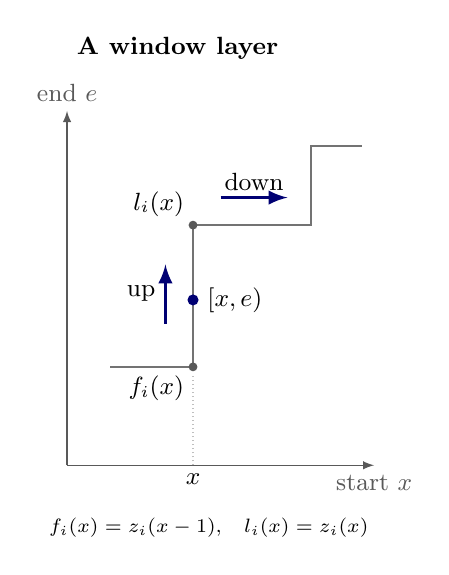
\begin{tikzpicture}[font=\small,>=latex,
  layer/.style={line width=.65pt,draw=black!55},
  connection/.style={line width=1.35pt,draw=blue!45!black},
  guide/.style={draw=black!25,densely dotted,line width=.45pt}]

  \begin{scope}[shift={(0,.75)}]
    \node[anchor=west,font=\small\bfseries] at (0,5.3) {A window layer};
    \draw[->,black!65] (0,0) -- (3.9,0) node[below] {start $x$};
    \draw[->,black!65] (0,0) -- (0,4.5) node[above] {end $e$};
    \draw[layer] (.55,1.25) -- (1.6,1.25) -- (1.6,3.05)
      -- (3.1,3.05) -- (3.1,4.05) -- (3.75,4.05);
    \fill[black!65] (1.6,1.25) circle (1.6pt);
    \fill[black!65] (1.6,3.05) circle (1.6pt);
    \node[anchor=north east,inner sep=3pt] at (1.6,1.25) {$f_i(x)$};
    \node[anchor=south east,inner sep=3pt] at (1.6,3.05) {$l_i(x)$};
    \draw[connection,->] (1.25,1.8) -- (1.25,2.55)
      node[midway,left,inner sep=3pt] {up};
    \draw[connection,->] (1.95,3.4) -- (2.8,3.4)
      node[midway,above,inner sep=2pt] {down};
    \fill[blue!45!black] (1.6,2.1) circle (2pt);
    \node[anchor=west,inner sep=5pt] at (1.6,2.1) {$[x,e)$};
    \draw[guide] (1.6,0) -- (1.6,1.17);
    \node[below,inner sep=3pt] at (1.6,0) {$x$};
    \node[anchor=north,align=center,font=\scriptsize] at (1.8,-.55)
      {$f_i(x)=z_i(x-1)$,\quad $l_i(x)=z_i(x)$};
  \end{scope}

\end{tikzpicture}

\caption{A layer in start--end coordinates. An up step appends a letter and increases the end; a down step deletes the first letter and increases the start. At start $x$, the layer visits every window $[x,e)$ between its first end $f_i(x)$ and its last end $l_i(x)$.}
\label{fig:layers}
\end{figure}

\subsection{Unblocked occurrences on layers}

Align a recorded occurrence of $s$ on a layer with a template $A$ containing $s$ at position zero. Call it blocked if the interval from the nearest left mismatch to the nearest right mismatch is itself recorded on that layer. Such a block automatically belongs to $V$, since it is a substring of a visited window.

\begin{lemma}[Matching window]\label{lem:matching-window}
Over all layers, the number of blocked occurrences of $s$ relative to $A$ is $B_A(s;m)$. Every unblocked occurrence is contained in an actual layer window that agrees with $A$ throughout.
\end{lemma}

\begin{proof}
Each recorded occurrence of a word $r$ counted in \eqref{eq:block-functional}, together with a counted placement of $s$ in it, gives a blocked occurrence. Conversely, the nearest mismatch pair uniquely determines $r$ and its placement. This correspondence commutes with translation by one layer turn, so it is a bijection also for the occurrences counted modulo that turn. \Cref{lem:recorded} gives the asserted count. Sorting layers did not change that lemma, since it preserved all base edges.

For the second assertion, write the selected occurrence as $[u,v)$. Its first containing window is reached by the up step with end $v$, so that window contains no right mismatch. If it has no left mismatch either, it suffices. Otherwise let $\ell<u$ be the nearest left mismatch. Follow the layer until a down step removes $\ell$; this happens while the windows still contain $[u,v)$, since their starts eventually reach $u$. No right mismatch can enter before that step: together with $\ell$ it would make the nearest-mismatch bracket a recorded interval, contrary to the occurrence being unblocked. The down step introduces no new letter. Immediately afterward no mismatch remains on either side, and the resulting actual window agrees throughout with $A$.
\end{proof}

In particular,
\begin{equation}\label{eq:unblocked-count}
m(s)-B_A(s;m)
\end{equation}
counts unblocked recorded occurrences. A layer whose entire text is the aligned template has no blocked occurrences relative to that template.

\subsection{Two periodicity facts}

Periodicity and extremal rotations also enter earlier superstring cycle-cover analyses~\cite{breslauer1997,mucha2013}. We prove the exact agreement and maximal-rotation statements needed here. Use the total order on $\Sigma$ induced by the encoded symbol labels. The lexicographic order of infinite forward words is determined by their first differing letter; equality means agreement at every nonnegative position. In a periodic group, a \emph{distinguished position} $t$ starts its lexicographically greatest forward rotation.

The agreement bound below uses only the weaker $p+q$ consequence of
Fine--Wilf periodicity~\cite{finewilf}; we retain its direct proof here.

\begin{lemma}[Agreement bounds]\label{lem:agreement}
Two distinct aligned periodic texts of periods $p,q$ agree on fewer than $p+q$ consecutive letters. If both have period $p$, they agree on fewer than $p$ consecutive letters.
\end{lemma}

\begin{proof}
Suppose that a period-$p$ text and a period-$q$ text agree on an interval of length $p+q$. For a full set of $q$ consecutive residues, both positions $i$ and $i+p$ lie in that interval. Equality with the first text therefore makes the second invariant under shift by $p$ at those residues, and $q$-periodicity extends this invariance everywhere. Both texts now have period $p$, and agreement for $p$ consecutive letters makes them equal. The same final observation proves the equal-period bound.
\end{proof}

\begin{lemma}[Maximal rotation]\label{lem:max-rotation}
Let $A$ have least period $p$, and let $t$ be distinguished. Let $D$ be a distinct aligned periodic text of period $q$, all of whose forward rotations are lexicographically at most the forward word of $A$ at $t$. Then $D$ and $A$ cannot agree on all $q$ positions starting at $t$.
\end{lemma}

\begin{proof}
Set $t=0$ by translating coordinates, and let $S$ be the forward word of $A$. It is at least its shift by $q$. If they are equal, $A$ has period $q$, and any period-$q$ text agreeing on the first $q$ letters is the identical aligned text.

Otherwise let $j\ge0$ be the first index at which $S(j)\ne S(j+q)$. Maximality gives $S(j)>S(j+q)$. Let $U$ repeat the first $q$ letters of $S$. The equalities $S(i)=S(i+q)$ for $i<j$ imply that $U$ and $S$ agree before index $j+q$. At that index,
\[
U(j+q)=U(j)=S(j)>S(j+q),
\]
so $U>S$. If $D$ agreed on the first $q$ letters, its forward word there would be $U$, contrary to the hypothesis on its rotations.
\end{proof}

\section{Connection operations}\label{sec:connections}

We now construct closed walks that touch existing layers at a cost charged to specified period budgets. We first give joins paid for entirely by the layers being attached, then an operation that also spends the receiving layer's budget. Each cross-text contact uses an actual word common to the two alignments; the band operation below is restricted to layers of one primitive-text group.

A collection of layers and added walks is \emph{rooted} if its graph support is connected to $\eps$. Connectivity is in the underlying undirected graph; every edge multiset we use is balanced. To \emph{touch} a layer means to share at least one of its graph vertices. Since all base edges remain, touching any vertex of a layer connects to every vertex of that layer.

\subsection{Following ordered windows}

\begin{lemma}[Ordered windows]\label{lem:ordered-windows}
Let $[a,b)$ and $[c,d)$ be windows in a common text over $\Sigma$, each spelling a word in $V$. If $a\le c$ and $b\le d$, there is a hierarchical-graph walk from the first word to the second of cost $d-b$. It visits a word of length at most $\max(0,b-c)$.

Consequently an ordered list of windows, with both starts and ends nondecreasing, can be followed at cost equal to the total increase in its ends. If its last window is a translate of the first by $h$ in a text of period dividing $h$, this is a closed walk of cost $h$.
\end{lemma}

\begin{proof}
If $c\le b$, delete the first $c-a$ letters, reaching $[c,b)$, and append through $d$. The words on the down path are suffixes of the first word; those on the up path are prefixes of the second. All belong to $V$, and the up cost is $d-b$.

If $c>b$, delete to the empty word. For each letter in the gap $[b,c)$, take an up step to that letter and a down step back to empty. Then build $[c,d)$. Single-letter words in the gap belong to $V$ because the text uses only $\Sigma$. The cost is $(c-b)+(d-c)=d-b$. Concatenating these constructions proves the assertions about lists and translates.
\end{proof}

In particular, a round trip from a vertex $s$ to $\eps$ and back costs $\len s$. Prescribed windows, rather than all intervals they sweep across, must belong to $V$; \Cref{lem:ordered-windows} supplies the intermediate vertices.

\begin{lemma}[Joining an ordered band]\label{lem:band}
Consider $k$ ordered layers from one primitive-text group of period $p$. At a start $t$, let $H$ be the top layer's first end and $E$ the bottom layer's last end. If $h$ is a nonnegative multiple of $p$ and $H-E\le h$, the layers can be joined together by a closed walk of cost at most $h$.
\end{lemma}

\begin{proof}
If $E\ge H$, every layer contains $[t,E)$: its first end is at most $H$ and its last end is at least $E$. No added walk is needed. Otherwise grow at start $t$ from end $E$ to $H$. Every layer has a vertical range intersecting $[E,H]$, so the growth touches them all. The endpoints are actual bottom and top vertices, and every intermediate word is a prefix of the top vertex. Finish by following to $[t+h,E+h)$, which is a period translate of the starting window. Since $E+h\ge H$, \Cref{lem:ordered-windows} gives a closed walk of cost $h$.
\end{proof}

\subsection{A collective outgoing link}

We call a chosen actual layer window, together with an alignment to a specified periodic text agreeing throughout it, a \emph{record}. A record on a receiving layer provides a vertex at which to attach layers following the other text. An ordinary \emph{link} spends only the attached layers' budgets. The following link attaches $k$ source layers at combined cost $kp$; it can therefore be planned without reserving any budget of the receiving layer. \Cref{fig:collective} illustrates its construction.

\begin{lemma}[Collective link]\label{lem:collective}
Consider $k$ ordered layers with a common period-$p$ text $A$, and put $K=kp$. Let $R=[a,b)$ spell a word in $V$ agreeing with $A$. Let $r_H=f_H(a)$ be the top layer's first end and $r_L=l_L(a)$ the bottom layer's last end. If
\begin{equation}\label{eq:collective-conditions}
r_H\le b+K,\qquad r_H-r_L\le K,
\qquad r_L+K\ge b,
\end{equation}
there is a cost-$K$ closed walk based at the word of $R$ that touches all $k$ layers.
\end{lemma}

\begin{proof}
Put $Y=\max(b,r_H)$. Then $b\le Y\le b+K$. For each constituent layer $i$,
\[
f_i(a)\le Y\le l_i(a)+K=l_i(a+K).
\]
Consequently its path meets height $Y$ at a start in $[a,a+K]$. More explicitly, choose the least such start $x_i$ with $z_i(x_i)\ge Y$. If $x_i=a$, then $z_i(a-1)=f_i(a)\le Y$; otherwise minimality gives $z_i(x_i-1)<Y$. Thus $[x_i,Y)$ is an actual vertex. Pointwise layer order makes the $x_i$ nondecreasing when layers are taken from top to bottom. The list from $R$ through these vertices to $R+K$ has nondecreasing starts and ends, and it closes because $K$ is a multiple of $p$. Apply \Cref{lem:ordered-windows}.
\end{proof}

\begin{figure}[tbp]
\centering
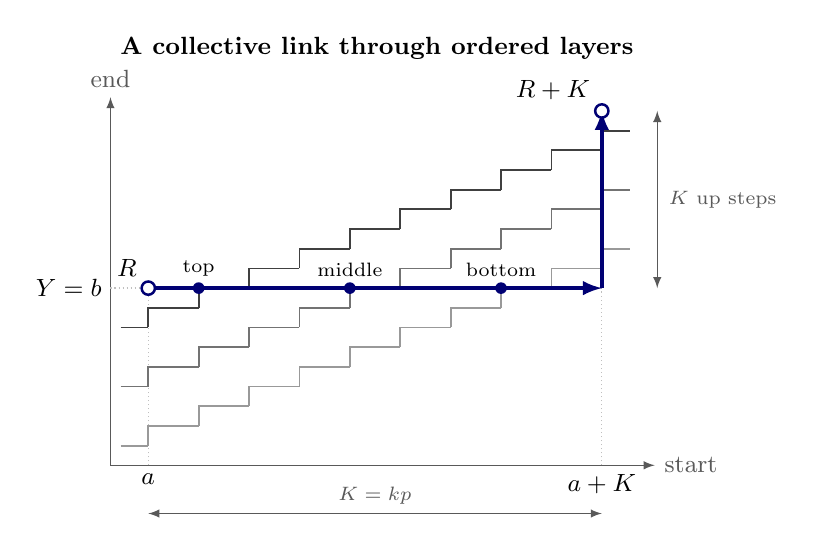
\begin{tikzpicture}[font=\small,>=latex,
  layer/.style={line width=.65pt,draw=black!55},
  connection/.style={line width=1.35pt,draw=blue!45!black},
  guide/.style={draw=black!25,densely dotted,line width=.45pt}]

  \begin{scope}[x=.64cm,y=.25cm]
    \node[anchor=west,font=\small\bfseries] at (-.75,24.2)
      {A collective link through ordered layers};
    \draw[->,black!65] (-.75,3) -- (10.05,3) node[right] {start};
    \draw[->,black!65] (-.75,3) -- (-.75,21.7) node[above] {end};
    \draw[guide] (0,3) -- (0,12);
    \draw[guide] (9,3) -- (9,12);
    \draw[guide] (-.75,12) -- (0,12);
    \node[left,inner sep=3pt] at (-.75,12) {$Y=b$};
    \node[below,inner sep=3pt] at (0,3) {$a$};
    \node[below,inner sep=3pt] at (9,3) {$a+K$};

    \foreach \c/\shade in {11/75,8/55,5/40} {
      \draw[layer,draw=black!\shade] (-.55,\c-1) -- (0,\c-1);
      \foreach \j in {0,...,8} {
        \draw[layer,draw=black!\shade]
          (\j,\j+\c-1) -- (\j,\j+\c) -- (\j+1,\j+\c);
      }
      \draw[layer,draw=black!\shade]
        (9,9+\c-1) -- (9,9+\c) -- (9.55,9+\c);
    }

    \draw[connection,->] (0,12) -- (9,12);
    \draw[connection,->] (9,12) -- (9,21);
    \foreach \j/\name in {1/top,4/middle,7/bottom} {
      \fill[blue!45!black] (\j,12) circle (2.1pt);
      \node[above,inner sep=4pt,font=\scriptsize] at (\j,12) {\name};
    }
    \filldraw[connection,fill=white,line width=.9pt] (0,12) circle (2.4pt);
    \node[above left,inner sep=4pt] at (0,12) {$R$};
    \filldraw[connection,fill=white,line width=.9pt] (9,21) circle (2.4pt);
    \node[above left,inner sep=4pt] at (9,21) {$R+K$};
    \draw[<->,black!65] (10.1,12) -- (10.1,21)
      node[midway,right,inner sep=4pt,align=left,font=\scriptsize]
      {$K$ up steps};
    \draw[<->,black!65] (0,.55) -- (9,.55)
      node[midway,above,inner sep=3pt,font=\scriptsize] {$K=kp$};
  \end{scope}
\end{tikzpicture}

\caption{A collective link in start--end coordinates. The common height $Y$ meets the ordered layers from top to bottom as the start increases. The endpoints $R$ and $R+K$ spell the same word in the source text, so the path closes at cost $K$. The illustration uses $Y=b$; the precise conditions are in \Cref{lem:collective}.}
\label{fig:collective}
\end{figure}

\subsection{Several requests at one host}

A \emph{request} reserves a source layer's budget for an operation at a receiving layer, called its \emph{host}. Unlike a link, this operation may also spend the host's budget. It handles all requests at that host together and roots every participating layer. In \Cref{sec:processing}, we will send requests only when the following hypotheses hold.

\begin{lemma}[Host requests]\label{lem:host}
Let a host layer have period $q$. On that layer choose actual windows $R_i=[a_i,b_i)$, indexed by a nonempty collection of distinct child groups. The text of child group $i$ has period $p_i$, is different up to translation from the host's text and from every other child group's text, and agrees with the host throughout $R_i$ in the chosen alignment.

For each $i$, one or more child layers request a connection at this same record. Each has a specified actual window $[a_i,e)$ satisfying
\begin{equation}\label{eq:request-condition}
a_i+p_i<e\le b_i-p_i.
\end{equation}
Its period-$p_i$ budget is reserved for the request. If the host's period-$q$ budget is also available, the host and all requesting layers can be rooted using at most these budgets.
\end{lemma}

\begin{proof}
We will spend the host budget on one closed excursion through contact words for the requesting layers. Requesters from all but one child group attach to those contacts using their own budgets. The requesters from the remaining group are touched directly by the host excursion, leaving one of their budgets to connect a contact shorter than their period to $\eps$.

By \Cref{lem:agreement},
\begin{equation}\label{eq:host-length}
b_i-a_i<p_i+q.
\end{equation}
If record $i$ is before record $l$ along a lift of the host path, their starts and ends are ordered. When $b_i>a_l$, their overlap is an agreement interval between two distinct child texts, so
\begin{equation}\label{eq:child-overlap}
b_i-a_l<p_i+p_l.
\end{equation}
If there is no overlap, the same strict inequality is immediate.

Choose an index $j$ of minimum $p_j$. Start at its record and order all other records before the next copy of it, translating coordinates by multiples of $q$ as needed. A shift by $\delta\in q\ZZ$ also transports that record's entire child coordinate system: replace its text by $A_i'(x)=A_i(x-\delta)$, its layer functions by $z_i'(x)=z_i(x-\delta)+\delta$, and its requester ends by $e+\delta$. This preserves all graph words, child periods, and budgets; the host text is unchanged because it is $q$-periodic. The same convention applies to the next copy of record $j$ when comparing overlaps. Put $T=a_j+q$. The order gives
\begin{equation}\label{eq:host-order}
a_j\le a_i\le T,\qquad b_j\le b_i\le b_j+q.
\end{equation}

To construct the host excursion, first visit all specified windows of the requesters at $j$ at start $a_j$, in increasing order of their ends $e$, and then visit $R_j$. For each later record $i$, the raw contact $[a_i+p_i,e)$ is obtained by deleting the first $p_i$ letters of the requester window and lies inside $R_i$. To place these contacts after $R_j$ and before the return at start $T$, we must keep their ends at least $b_j$ and their starts at most $T$. Accordingly, replace the raw contact by
\begin{equation}\label{eq:host-target}
Q_{i,e}=[s_i,h_{i,e})
=[\min(a_i+p_i,T),\max(e,b_j)).
\end{equation}
Visit these targets in record order and, within each record, in increasing order of $e$. Finally return to the first requester window translated by $q$.

For earlier $i$ and later $l$, \eqref{eq:request-condition} and \eqref{eq:child-overlap} give
\[
a_i+p_i<e_i\le b_i-p_i<a_l+p_l<e_l.
\]
Thus the raw targets have ordered starts and ends. The monotone operations in \eqref{eq:host-target} preserve this order. By \eqref{eq:host-order}, each modified target remains inside its record $R_i$, and it is nonempty because $s_i\le a_i+p_i<e\le h_{i,e}$. It therefore spells a word in $V$ and matches child text $i$.

Applying \eqref{eq:child-overlap} to $i$ and the next occurrence of $j$ gives
\[
b_i-T<p_i+p_j.
\]
Together with \eqref{eq:host-length}, this implies
\begin{equation}\label{eq:host-short-end}
e\le b_i-p_i<T+p_j,\qquad b_j<T+p_j,
\qquad h_{i,e}<T+p_j.
\end{equation}
If $e_0$ is the first requester end at $j$, then $e_0>a_j+p_j$, so the final translated window $[T,e_0+q)$ has end greater than $T+p_j$. The whole list is therefore ordered. Its closed excursion costs $q$ by \Cref{lem:ordered-windows}. On its final transition it reaches a vertex of length less than $p_j$. If there are no later records, the same conclusion follows using $b_j<T+p_j$.

It remains to attach the other requesters and root the piece. For a requester at $i\ne j$, the target satisfies
\begin{equation}\label{eq:target-child-range}
a_i\le s_i\le a_i+p_i,
\qquad e\le h_{i,e}\le e+p_i.
\end{equation}
Only the upper end bound needs an additional check. Here the choice of a minimum period $p_j$ is used: if $h_{i,e}=b_j$, then
\[
b_j<a_i+p_j+p_i\le a_i+2p_i<e+p_i.
\]
In child text $i$, follow the ordered list
\[
Q_{i,e},\quad[a_i+p_i,e+p_i),\quad Q_{i,e}+p_i.
\]
The middle word is a period translate of the actual requester vertex; the last word equals the first. The inequalities \eqref{eq:target-child-range} make the list ordered. Its cost-$p_i$ loop attaches this requester at the target. Do this separately for all requesters with $i\ne j$.

The requesters at $j$ were already touched in the initial vertical part, so their budgets have not been spent. Use one of their budgets $p_j$ to connect the short contact from \eqref{eq:host-short-end} to $\eps$. The host is touched at $R_j$, all requesters are attached, and the expenditure is at most the host budget plus all requester budgets.
\end{proof}

\section{Processing the period groups}\label{sec:processing}

We now give the connection procedure. Process the primitive-text groups in increasing order of least period, breaking ties by the lexicographically least rotation of their primitive texts. Requests reserve budgets and are fulfilled when their host group is processed. Ordinary links are planned now and finalized in \Cref{sec:cycles}. Every record and every layer in these plans refers to the fixed base decomposition from \Cref{lem:layers}. For bookkeeping, mark a layer rooted when a stated operation explicitly roots it. Incidental connections to $\eps$ do not change these marks or budget assignments.

\subsection{Incoming requests and a baseline}

At entry to a group of period $p$, fulfill all requests received by each recipient layer in one application of \Cref{lem:host}. We will prove below that every requester has smaller period, and that a child group sends requests using only one record on one recipient layer. These are precisely the facts needed to apply that lemma with fresh recipient budgets.

Every recipient has an actual vertex of length less than $2p$: its record with a child of period $r<p$ has length less than $p+r$ by \Cref{lem:agreement}. If there are recipients, choose their highest layer as a \emph{baseline}. They and their requesters have already been rooted.

Each remaining layer below the baseline can be rooted with its own budget $p$. If it has a vertex of length at most $p$, take a round trip through $\eps$. Otherwise choose a baseline vertex $S=[a,h)$ of length less than $2p$. A lower layer has a vertex $[a,e)$ with
\[
p<e-a\le h-a<2p.
\]
For example, take $e=\min(l_i(a),h)$; pointwise ordering ensures this lies in its vertical range. The windows
\[
[a,h),\qquad[a+p,e+p),\qquad[a+p,h+p)
\]
are ordered because $h<a+2p<e+p$. Their cost-$p$ closed walk touches the lower layer and the rooted baseline. Recipient layers themselves need no further budget.

Let $n$ be the number of layers above the baseline, or the entire number in the group when there is no baseline. Their budgets are all still available. If $n=0$, proceed to the next group.

\subsection{Easy connections for the upper layers}

Use a distinguished position $t$ of the group's text $A$, and put
\[
H=f_H(t),
\]
the top layer's first end at that start. If $H-t\le np$, a round trip from $\eps$ through $[t,H)$ costs at most $np$. Its up path touches every upper layer, since every such layer has first end at most $H$. This roots them all.

If a baseline exists and its last end $E$ at $t$ satisfies $E\ge H-np$, \Cref{lem:band}, including the baseline as the bottom layer and taking $h=np$, joins it to all upper layers within their combined budget. This also roots them all.

It remains to handle the case
\begin{equation}\label{eq:hard-case}
H>t+np,
\qquad l_{\mathrm{base}}(t)<H-np
\quad\text{when a baseline exists}.
\end{equation}

\subsection{Forcing a record on another aligned text}

The count rule will supply $k+1$ unblocked occurrences of a word obtained by shortening the top vertex by $kp$. We choose $k$ so that at most $k$ of those occurrences can have the present full-text alignment. The same choice must keep the top $k$ layers close enough to join for at most $(k-1)p$, leaving one period of their combined budget available. The following threshold search gives both properties.

Starting at $k=1$, increase $k$ while the number of layers of this group satisfying
\[
l_i(t)\ge H-kp
\]
exceeds $k$. Stop at the first failure of this test and set $K=kp$.

\begin{lemma}\label{lem:choose-k}
This procedure stops with $1\le k\le n$. If $L_*$ is the lowest of the top $k$ layers, then
\begin{align}
l_{L_*}(t)&\ge H-(k-1)p,\label{eq:sharp-band}\\
f_H(x)-l_{L_*}(x)&\le K\qquad(x\in\ZZ).\label{eq:wide-band}
\end{align}
At most $k$ recorded occurrences of $w=A[t:H-K)$ have a full-text alignment identical to $A$.
\end{lemma}

\begin{proof}
For $k\le n$, layers at or below the baseline do not qualify, by \eqref{eq:hard-case}. Thus the process stops by $n$. If $k=1$, the top last end is at least its first end $H$. If $k>1$, reaching $k$ means that at least $k$ layers qualified at the previous threshold $H-(k-1)p$. Pointwise ordering gives \eqref{eq:sharp-band}.

For any $x$, choose its translate $x'$ modulo $p$ in $(t-p,t]$. Then
\[
f_H(x')\le H,
\qquad l_{L_*}(x')\ge l_{L_*}(t)-p.
\]
Their difference is invariant under period translation, proving \eqref{eq:wide-band}.

By \eqref{eq:hard-case}, $H-K>t$, so $w$ is nonempty. Each primitive layer has exactly one position residue whose full-text alignment agrees with $A$: the shifts preserving its text are exactly the multiples of $p$. At that alignment, $w$ is recorded exactly when $l_i(t)\ge H-K$. At most $k$ layers satisfy this inequality when the test stops. Other primitive-text groups have no identical full-text alignment.
\end{proof}

Apply the count rule \eqref{eq:period-rule}, with origin shifted to $t$, to the actual vertex word
\[
v=A[t:H),\qquad w=A[t:H-K).
\]
The top layer records an unblocked occurrence of $v$ in its own text. By \eqref{eq:unblocked-count}, the trigger holds, and the rule gives at least $k+1$ unblocked occurrences of $w$. \Cref{lem:choose-k} leaves at least one on a layer $D$ whose aligned text differs from $A$. A different phase of this same group is allowed.

Choose one such occurrence. \Cref{lem:matching-window} gives an actual window $R=[a,b)$ on $D$, agreeing with $A$ throughout and containing the specified interval $[t,H-K)$. Let $q$ be the least period of $D$. Thus
\begin{equation}\label{eq:chosen-record}
a\le t,
\qquad b\ge H-K,
\qquad b-a<p+q.
\end{equation}
If $D$ belongs to this same primitive-text group, then
\begin{equation}\label{eq:same-group-record}
b-a<p.
\end{equation}
The strict length bounds follow from \Cref{lem:agreement}. Use this \emph{one} chosen record for every subsequent connection from this processed group.

\subsection{Distributing the remaining budgets}

At start $a$, put $r_H=f_H(a)$ and $r_L=l_{L_*}(a)$. Monotonicity, \eqref{eq:wide-band}, and \eqref{eq:chosen-record} give
\begin{equation}\label{eq:block-preconditions}
r_H-r_L\le K,
\qquad r_H\le H\le b+K.
\end{equation}

\paragraph{The collective case.}
If $r_L+K\ge b$, make the top $k$ layers one \emph{collective block}. Plan the link in \Cref{lem:collective} from these layers to $D$ at $R$, reserving their combined budget $K$. Here a collective block is allowed to have $k=1$; its plan is still the collective construction. If the test fails, do not make the block. In that event,
\begin{equation}\label{eq:failed-collective}
r_H\le r_L+K<b.
\end{equation}

\paragraph{The individual cases.}
Handle every upper layer not placed in that collective block separately. Its first end at $a$ is at most $b$. When the collective test failed, this follows from \eqref{eq:failed-collective}; a layer below the top $k$ has
\[
f_i(a)\le l_i(t)<H-K\le b
\]
by the stopping rule and $a\le t$.

For such a layer, do exactly one of the following.
\begin{enumerate}[label=\textup{(\roman*)}]
\item If some vertex has length at most $p$, root the layer by a round trip through $\eps$ using at most its budget.
\item If all its vertex lengths exceed $p$ and
\begin{equation}\label{eq:single-test}
l_i(a)+p\ge b,
\end{equation}
make it an \emph{individual block} with a planned link to $D$ at $R$. At start $a+p$, its vertical range intersects $[b,b+p]$, since
\[
f_i(a+p)=f_i(a)+p\le b+p,
\qquad l_i(a+p)=l_i(a)+p\ge b.
\]
Choose an actual end $e'\in[b,b+p]$ there and follow
\begin{equation}\label{eq:individual-list}
[a,b),\qquad[a+p,e'),\qquad[a+p,b+p).
\end{equation}
This is a cost-$p$ closed walk in $A$ touching the layer. Its incoming transition to start $a+p$ reaches a word of length at most
\begin{equation}\label{eq:single-short}
\max(0,b-a-p)\le q,
\end{equation}
by \eqref{eq:chosen-record} and \Cref{lem:ordered-windows}. Reserve this layer's budget for that link.
\item Otherwise reserve the layer's budget $p$ and send a request to $D$ at the same record $R$. Its first end $e=f_i(a)$ satisfies
\begin{equation}\label{eq:outgoing-request}
a+p<e\le l_i(a)<b-p.
\end{equation}
This is the condition of \Cref{lem:host}. In particular $b-a>2p$; combining this with $b-a<p+q$ gives $q>p$. The recipient group will therefore be processed later.
\end{enumerate}

This verifies the promised hypotheses for incoming requests. They always go to strictly larger periods, and a child group uses just one record on one recipient layer, even if several of its layers request there. Ordinary planned links consume no recipient budget. When a recipient is processed, its own budget and all reserved requester budgets are available. After \Cref{lem:host} is applied, those layers are rooted and do not enter any outgoing block.

\begin{proposition}\label{prop:partition}
After all groups have been processed, every layer is either marked rooted or belongs to exactly one outgoing block. These two classes are disjoint. Each block consists of layers from one primitive-text group and targets a single actual layer. Its total budget remains reserved for its planned link. A collective block of $k$ layers and period $p$ also satisfies \eqref{eq:sharp-band} at its distinguished position; an individual block consists of one layer.
\end{proposition}

\begin{proof}
Incoming requests use disjoint requester budgets, and each recipient budget is spent only when its group is processed. The baseline step uses only budgets of remaining lower layers. The easy upper-layer branches use at most the combined budgets of the upper layers and finish them. In the remaining branch, the collective case and the individual cases partition those upper layers. Each request is eventually fulfilled, because its recipient is processed later. The layers not marked rooted by a direct operation or a fulfilled request are precisely the outgoing blocks. Their links have only been planned, so their budgets are unspent. The asserted inequality for collective blocks is \eqref{eq:sharp-band}.
\end{proof}

\section{Opening cycles of planned links}\label{sec:cycles}

It remains to execute the plans in \Cref{prop:partition}. Regard a block as one node and map its target layer to the block containing that layer, or to a rooted sink if the target is marked rooted. Each nonsink node has exactly one outgoing edge. A component therefore reaches a rooted sink or contains one directed cycle. Additional graph intersections between layers can only help; the following argument does not need them to be recorded by this bookkeeping graph.

\begin{lemma}[One free period]\label{lem:free-period}
A block of $k$ layers and period $p$ can be joined internally, in place of its outgoing link, for cost at most $(k-1)p$. Thus this replacement leaves at least $p$ of its total budget available.
\end{lemma}

\begin{proof}
For an individual block, or any block with $k=1$, no internal addition is needed. For a collective block, \eqref{eq:sharp-band} gives
\[
f_H(t)-l_{L_*}(t)\le(k-1)p.
\]
Apply \Cref{lem:band} with $h=(k-1)p$.
\end{proof}

\begin{lemma}[A short contact on a maximal link]\label{lem:cycle-contact}
On a directed cycle of blocks, choose a block whose group's distinguished forward rotation is lexicographically greatest. If its target layer has period $q$, its planned outgoing link can be realized within its reserved budget so that the resulting connected piece contains a vertex of length at most $q$.
\end{lemma}

\begin{proof}
If the plan is an individual link, \eqref{eq:single-short} already gives the contact. For a collective plan with $k$ source layers of period $p$, put $K=kp$. Recall that $t$ is distinguished, $H=f_H(t)$, and the target record $R=[a,b)$ agrees with the source text and satisfies
\[
a\le t<H-K\le b,\qquad b-a<p+q.
\]
If any constituent layer already contains a vertex of length at most $q$, the ordinary collective link connects that vertex to the target and to all other constituents, so it suffices.

Otherwise every vertex on every constituent layer has length greater than $q$. Every forward rotation of the target's text is at most its own distinguished rotation, and hence at most the selected block's distinguished rotation. The target alignment is different from the source alignment by construction. If $b-t\ge q$, agreement on $R$ would include all $q$ positions starting at $t$, contrary to \Cref{lem:max-rotation}. Thus
\begin{equation}\label{eq:cycle-agreement}
b-t<q.
\end{equation}
Put $x=\min(t,a+K)$. We have $a\le x\le a+K$ and $x\le t<b$. If $x=t$, \eqref{eq:cycle-agreement} gives $b-x<q$. If $x=a+K<t$, then
\[
b-x=b-a-K<p+q-K\le q.
\]
Thus $[x,b)$ is a suffix of $R$ of length less than $q$.

At start $x$, every constituent layer's first end exceeds $b$, because its corresponding word has length greater than $q>b-x$. These first ends are all at most $H$: they are no greater than the top first end at $x$, which is at most its first end at $t$. Let $F=f_H(x)$. Then $b<F\le H\le b+K$. Descend from $R$ to $[x,b)$ and grow at start $x$ to $[x,F)$. This growth touches every constituent at its first end, and all intermediate words are prefixes of the actual top-layer vertex. Finish at $R+K$.

In summary, the prescribed list is
\begin{equation}\label{eq:cycle-list}
[a,b),\qquad[x,b),\qquad[x,F),\qquad[a+K,b+K).
\end{equation}
Its starts and ends are nondecreasing. Every prescribed word is in $V$, and the last equals the first in the period-$p$ source text. \Cref{lem:ordered-windows} makes it a cost-$K$ closed walk, with the short contact $[x,b)$.
\end{proof}

\begin{theorem}[Connecting the base graph]\label{thm:connection}
The base graph can be connected to $\eps$ by adding closed walks of total up cost at most $W$.
\end{theorem}

\begin{proof}
Use the group procedure of \Cref{sec:processing}. Its fulfilled requests and direct connections have already rooted the layers outside outgoing blocks within their assigned budgets. Consider the remaining functional graph.

For a cycle consisting of one block, its target layer belongs to the same block, hence to the same primitive-text group. The chosen record has a different alignment, so \eqref{eq:same-group-record} gives $\len R<p$. Replace the outgoing link by the internal joining of \Cref{lem:free-period}. The target layer, and therefore $R$, lies in this joined piece. The freed budget $p$ pays for a round trip between $R$ and $\eps$.

For a cycle of at least two blocks, choose the outgoing link in \Cref{lem:cycle-contact}; write $q$ for its target block's period. Retain that selected link, with its contact of length at most $q$. Omit the \emph{target block's} outgoing link, replacing it by internal joining. This frees $q$ by \Cref{lem:free-period}. The selected link and the omitted link are different, since the cycle has length greater than one. All other cycle links, together with the target's internal joining, connect the entire cycle into one piece. Use the freed $q$ to root the short contact. \Cref{fig:cycles} illustrates this choice of the omitted edge.

Distinct directed cycles have disjoint blocks, so these replacements do not compete for budgets. Finally execute the links leading into the rooted pieces, in increasing distance from a root or an opened cycle. Each attaches its source block using only that source's reserved budget. All layers are now rooted.

Every addition is a closed walk. The initial layer budgets sum to $W$, and each budget was used only in its assigned operation or its cycle replacement. The total added up cost is therefore at most $W$.
\end{proof}

\begin{figure}[t]
\centering
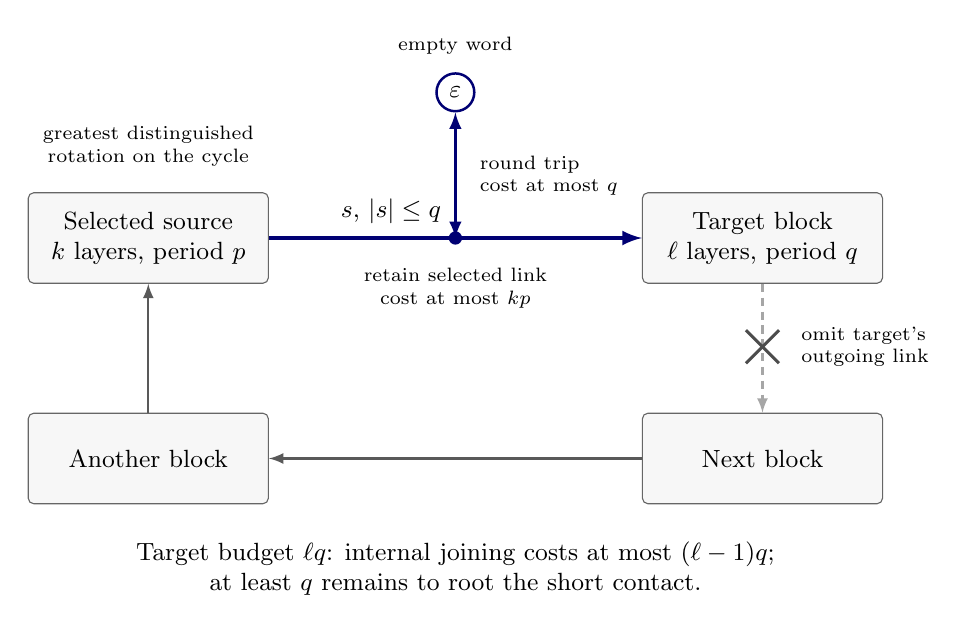
\begin{tikzpicture}[font=\small,>=latex,
  block/.style={draw=black!60,rounded corners=2pt,fill=black!3,
    minimum width=3.05cm,minimum height=1.15cm,align=center,inner sep=5pt},
  link/.style={->,draw=black!65,line width=.8pt},
  selected/.style={->,draw=blue!45!black,line width=1.4pt}]
  \node[block] (source) at (0,2.8)
    {Selected source\\$k$ layers, period $p$};
  \node[block] (target) at (7.8,2.8)
    {Target block\\$\ell$ layers, period $q$};
  \node[block] (next) at (7.8,0)
    {Next block};
  \node[block] (last) at (0,0)
    {Another block};

  \draw[selected] (source.east) -- (target.west)
    node[midway,below=7pt,align=center,font=\scriptsize]
      {retain selected link\\cost at most $kp$};
  \draw[link] (next.west) -- (last.east);
  \draw[link] (last.north) -- (source.south);

  \draw[->,draw=black!35,densely dashed,line width=.8pt]
    (target.south) -- (next.north);
  \draw[black!70,line width=1.1pt] (7.59,1.21) -- (8.01,1.63);
  \draw[black!70,line width=1.1pt] (7.59,1.63) -- (8.01,1.21);
  \node[anchor=west,align=left,font=\scriptsize] at (8.17,1.42)
    {omit target's\\outgoing link};

  \coordinate (contact) at (3.9,2.8);
  \fill[blue!45!black] (contact) circle (2.4pt);
  \node[anchor=south east,inner sep=5pt] at (contact) {$s$, $|s|\le q$};
  \node[circle,draw=blue!45!black,fill=white,line width=.9pt,
    minimum size=.48cm,inner sep=2pt] (root) at (3.9,4.65) {$\varepsilon$};
  \node[above=3pt,font=\scriptsize] at (root.north) {empty word};
  \draw[<->,draw=blue!45!black,line width=1.05pt]
    (contact) -- (root.south)
    node[midway,right=5pt,align=left,font=\scriptsize]
      {round trip\\cost at most $q$};

  \node[above=6pt,align=center,font=\scriptsize] at (source.north)
    {greatest distinguished\\rotation on the cycle};
  \node[anchor=north,align=center] at (3.9,-.93)
    {Target budget $\ell q$: internal joining costs at most $(\ell-1)q$;\\
     at least $q$ remains to root the short contact.};
\end{tikzpicture}

\caption{Opening a directed cycle of planned block links. Keep a link whose source has maximal distinguished rotation and realize it with a contact of length at most $q$, the target's period. Omit the target block's outgoing link and join that block internally, freeing $q$ to connect the contact to the empty word. Arrows between blocks represent planned dependencies, each realized by a closed walk; the dot is a contact vertex, not an extra block.}
\label{fig:cycles}
\end{figure}

\section{Polynomial time and the output string}\label{sec:algorithm}

\begin{proof}[Proof of \Cref{thm:main}]
Parse and preprocess the explicit input in time polynomial in its encoded size $N$. This handles the empty instance and preserves the optimum otherwise. In the nonempty case, construct the counts and base graph of \Cref{sec:counts}. By \Cref{lem:counts,lem:base}, its cost is $W\le\OPT(\mathcal S)$ and it contains every required vertex. Apply \Cref{thm:connection}. The resulting graph is balanced, its used support is connected, it includes $\eps$, and its total up cost is at most $2W$.

A finite balanced directed multigraph with connected used support has a closed Euler tour from any used vertex. One may obtain it by following unused edges until a closed walk is formed, and splicing further closed walks at visited vertices until all edges have been used. Balance prevents an unfinished walk from stopping away from its starting point, and connectivity ensures that any unused edges can eventually be reached for a splice.

Start such a tour at $\eps$ and write down the appended letter at each up step. At every step, the current vertex word is a suffix of the string written so far: an up step appends a letter to both, and a down step removes the first letter of the vertex. Every required string is visited and therefore occurs as a substring of the output. Its length is the number of up steps, at most $2W\le2\OPT(\mathcal S)$.

We finish by verifying that all preceding constructions are deterministic polynomial-time operations on explicit finite data. Order encoded symbols, input strings, substring vertices, layers, records, and edge copies by their explicit codes and stable indices. At every finite choice in the construction, including walk decompositions, eligible records, tied extrema, and Euler splices, take the first admissible item in this order. Comparisons and output of variable-width symbol codes are charged their bit cost; no unit-cost operation on an unbounded label or random choice is used.

\paragraph{Counts and graph.}
There are $O(L^2)$ words in $V$, each of length at most $L\le N$; store their explicit labels or interned identifiers in a dictionary. For each $v$, enumerate $1\le p<\len v$ and $k\ge1$ with $kp<\len v$. The period-$p$ template is specified by $v[0:p)$, and testing whether it matches $v$ takes polynomial time. Thus all rules \eqref{eq:period-rule} form a polynomial list. Each blocking functional is evaluated by enumerating $r\in V$ and the possible placements in \eqref{eq:block-interior}--\eqref{eq:block-ends}. The descending count recursion uses only such evaluations and integer maxima. By \Cref{lem:counts}, all counts are at most $L$, so their bit lengths are polynomial as well.

By \Cref{lem:base}, the explicit base graph has exactly $2W\le2L$ edges with multiplicity; adjacency lists retain individual edge-copy IDs. Its closed-walk decomposition can be found by finite edge traversals. Primitive periods, alignments of texts, and sorted passage lists can be found by direct string comparisons and sorting. The total number of primitive layer phases is the sum of their periods, namely $W$. Store each layer by its primitive period word, one period of exit-end values $z(x)$, and a stable ID; \eqref{eq:layer-properties} recovers other coordinates without enumerating an infinite text.

\paragraph{Records and connections.}
The first and last ends of a layer, its minimum vertex length, and the distinguished rotation of its text can be computed from one period. Equality or lexicographic comparison of two periodic texts requires at most the sum of their periods to find a difference, by \Cref{lem:agreement}. Normalize the start of each considered periodic record to one turn, translating its aligned child coordinates with it as in \Cref{lem:host}. Each actual window labels a substring of length at most $L$, so the resulting coordinates, lengths, and end differences have polynomial bit length. A record is stored by layer ID, phase, normalized start and end, and its alignment.

The search for a record in \Cref{sec:processing} is also finite. A period-$p$ layer has $p$ up steps and $p$ down steps, hence $2p$ window visits per turn, counting the initial vertex but not its repeated final copy. There are therefore $2W$ such visits over all layers. For the specified $w$ and template $A$, enumerate these actual windows and all placements of $w$ in them. Align each placement with $[t,H-K)$, reject a candidate whose complete aligned text equals $A$, and retain one whose entire window agrees with $A$. There are at most $2WL$ candidates. The count rule and \Cref{lem:choose-k,lem:matching-window} guarantee a covering window on a different aligned text, so this search succeeds.

The host operations, collective links, and internal joins require only ordered lists of windows and the paths of \Cref{lem:ordered-windows}; materialize these as explicit edge lists. Finding the intersections used in \Cref{lem:collective} is a scan along at most $K=kp$ units of start coordinate, with $K$ no larger than the group's budget and hence at most $W$. Group processing and the final outgoing-block functional graph likewise use polynomially many layers and blocks.

\paragraph{Materializing the answer.}
Every added walk is closed, so its number of down steps equals its number of up steps. The total added up cost is at most $W$, and hence the final graph has at most $4W\le4L$ edges with multiplicity. Its explicit construction and Euler traversal are polynomial. This proves both the approximation guarantee and the running-time assertion.
\end{proof}

\begingroup\small
\begin{thebibliography}{99}

\bibitem{blum1994}
Avrim Blum, Tao Jiang, Ming Li, John Tromp, and Mihalis Yannakakis.
\newblock Linear approximation of shortest superstrings.
\newblock \emph{Journal of the ACM}, 41(4):630--647, 1994.
\newblock \href{https://doi.org/10.1145/179812.179818}{doi:10.1145/179812.179818}.

\bibitem{breslauer1997}
Dany Breslauer, Tao Jiang, and Zhigen Jiang.
\newblock Rotations of periodic strings and short superstrings.
\newblock \emph{Journal of Algorithms}, 24(2):340--353, 1997.
\newblock \href{https://doi.org/10.1006/jagm.1997.0861}{doi:10.1006/jagm.1997.0861}.

\bibitem{cycle2026}
Nikolai Chukhin, Alexander S. Kulikov, Ivan Mihajlin, and Alexander Smal.
\newblock A tight cycle-cover inequality for shortest common superstring.
\newblock \emph{Electronic Colloquium on Computational Complexity},
Report TR26-157, August 2026. Preprint.
\newblock \url{https://eccc.weizmann.ac.il/report/2026/157/}.

\bibitem{emv2023}
Matthias Englert, Nicolaos Matsakis, and Pavel Vesel\'{y}.
\newblock Approximation guarantees for shortest superstrings: Simpler and better.
\newblock In \emph{34th International Symposium on Algorithms and
Computation (ISAAC 2023)}, volume 283 of \emph{LIPIcs}, pages 29:1--29:17, 2023.
\newblock \href{https://doi.org/10.4230/LIPIcs.ISAAC.2023.29}{doi:10.4230/LIPIcs.ISAAC.2023.29}.

\bibitem{finewilf}
N. J. Fine and H. S. Wilf.
\newblock Uniqueness theorems for periodic functions.
\newblock \emph{Proceedings of the American Mathematical Society}, 16:109--114, 1965.
\newblock \href{https://doi.org/10.1090/S0002-9939-1965-0174934-9}{doi:10.1090/S0002-9939-1965-0174934-9}.

\bibitem{collapsing2020}
Alexander Golovnev, Alexander S. Kulikov, Alexander Logunov,
Ivan Mihajlin, and Maksim Nikolaev.
\newblock Collapsing superstring conjecture.
\newblock In \emph{APPROX/RANDOM 2019}, volume 145 of \emph{LIPIcs},
article 26, 2019.
\newblock \href{https://doi.org/10.4230/LIPIcs.APPROX-RANDOM.2019.26}{doi:10.4230/LIPIcs.APPROX-RANDOM.2019.26};
\href{https://arxiv.org/abs/1809.08669v3}{revised arXiv version, 4 June 2020}.

\bibitem{golovnev2014}
Alexander Golovnev, Alexander S. Kulikov, and Ivan Mihajlin.
\newblock Solving {SCS} for bounded length strings in fewer than $2^n$ steps.
\newblock \emph{Information Processing Letters}, 114(8):421--425, 2014.
\newblock \href{https://doi.org/10.1016/j.ipl.2014.03.004}{doi:10.1016/j.ipl.2014.03.004}.

\bibitem{mucha2013}
Marcin Mucha.
\newblock Lyndon words and short superstrings.
\newblock In \emph{Proceedings of SODA 2013}, pages 958--972, 2013.
\newblock \href{https://doi.org/10.1137/1.9781611973105.69}{doi:10.1137/1.9781611973105.69}.

\bibitem{greedy2026}
Hiroki Shibata.
\newblock Disproving the greedy superstring conjecture.
\newblock \href{https://arxiv.org/abs/2609.01365v1}{arXiv:2609.01365v1},
1 September 2026. Preprint.

\bibitem{sweedyk1999}
Z. Sweedyk.
\newblock A 2.5-approximation algorithm for shortest superstring.
\newblock \emph{SIAM Journal on Computing}, 29(3):954--986, 1999.
\newblock \href{https://doi.org/10.1137/S0097539796324661}{doi:10.1137/S0097539796324661}.

\bibitem{tarhio1988}
Jorma Tarhio and Esko Ukkonen.
\newblock A greedy approximation algorithm for constructing shortest common superstrings.
\newblock \emph{Theoretical Computer Science}, 57(1):131--145, 1988.
\newblock \href{https://doi.org/10.1016/0304-3975(88)90167-3}{doi:10.1016/0304-3975(88)90167-3}.

\end{thebibliography}
\endgroup

\end{document}
